\section{Basics of \gls{lidar}}
\label{sec:chap_lidar_basics}

\gls{lidar} is a technology based on laser time of flight to measure distances. \citet{lidar_basics} present the physical details as well as the pros and cons of three time of flight commonly used in \gls{lidar}s, namely the pulsed, phase-shift and frequency modulated continuous wave. In the context of our research, we focus more on higher level concepts that could cause sensor readings to be erroneous for modeling 3D environments or objects. Beams emitted by a \gls{lidar} have a given with width and angle at source. This cause the beam two-dimensional pattern on the target to grow with distance. Once the light hit the target, it bounces back to the sensor which will extract the range information out of it. The signal received by the sensor can be seen as a waveform and its shape highly depends on the target surface. Processing data from smooth surfaces is generally straightforward, but multi-modal waveforms caused by partially transparent material, fog, dust, small objects and edges are ambiguous. Figure~\ref{fig:lidar_basics} depict laser beam hitting different targets along with the resulting waveforms. While some \gls{lidar}s provide full waveform, they generally only output a single or few echoes and the inference method differs from sensor to sensor (e.g., using the first or last maximum, using the mean). For this reason, it is important to determine whether the sensor of your choice is well suited to your needs. Figure~\ref{fig:shadow_points} show how reading errors affect the 3D representation of the environment surrounding the robot. Note that it is possible to obtain a complete 3D representation as shown in Figure through a pivoting internal mirror to the sensor and / or an external motor rotating the sensor.

\begin{figure}[htpb]
    \centering
    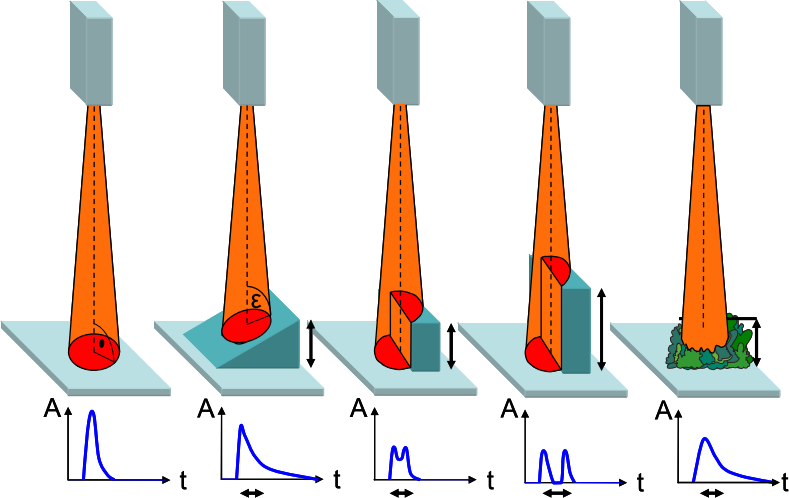
\includegraphics[width=0.8\linewidth]{img/chap_lidar/waveforms.png}
    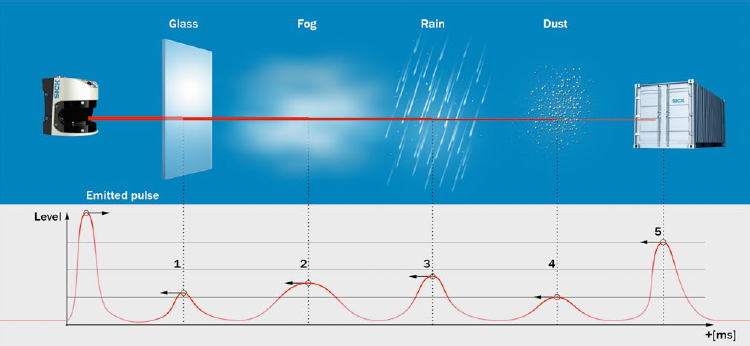
\includegraphics[width=0.8\linewidth]{img/chap_lidar/waveforms2.png}
    \caption{\todo{Write some caption and add the SICK ref} From \citet{lidar_figure1} Yo dang (http://www.robotsinsearch.com/products/lms500-21000-lite)}
    \label{fig:lidar_basics}
\end{figure}

\begin{figure}[htpb]
    \centering
    %\includegraphics[width=0.8\linewidth]{img/chap_lidar/shadow_points.png}
    \caption{\todo{Get some picture of the husky along with the erroneous point cloud} Some points appear around the robot forming a nonexistent conical structure}
    \label{fig:shadow_points}
\end{figure}
